\documentclass{beamer}
\usepackage{amsmath}
\title{Resource Access Planning:  Healthcare - Electricity}
\author{Chris Natali}
\institute{Modi Labs at Columbia University}
\date{May 22, 2013}
\begin{document}

\begin{frame}{Resource Access}

  What: 
  \begin{itemize}
  \item[] Healthcare:  Clinics, Hospitals...
  \item[] Education:  Schools (Primary, Secondary, etc)
  \item[] Water:  Wells, Pumps, Taps...
  \item[] Electricity:  Generators, Transformers, LV/MV line...
  \end{itemize}
 
  \bigskip 

  Where: 
  \begin{itemize}
  \item[] Access is limited
  \item[] Sub-Saharan Africa (minus South Africa)
  \item[] India, Indonesia
  \item[] Rural regions
  \end{itemize}


\end{frame}


\begin{frame}{Process}

  How: 
  \begin{itemize}
  \item[] Collect Data:  From existing sources, via Formhub, other tools
  \item[] Frame it in Economic terms (Supply, Demand)
  \item[] Assess "Gaps" in supply 
  \item[] Develop plan to fill the gaps
  \end{itemize}

  \bigskip 
  Healthcare:  Facility Planning demo

  \bigskip 
  Sea Urchin Story (Healthcare is more effective with Electricity)

\end{frame}

\begin{frame}{Electrification Planning}
  
  Inputs: 
  \begin{itemize}
  \item[] Supply:  Existing grid
  \item[] Demand:  Settlements to be electrified
  \item[] Model Parameters:  Generation, Distribution costs, Growth/Demand curves
  \end{itemize}

  \bigskip 

  Outputs: 
  \begin{itemize}
  \item[] Electrification selection per settlement (Solar, Diesel, Grid)
  \item[] Costs (settlement and regional level)
  \end{itemize}

\end{frame}

\begin{frame}{Data Collection System}
  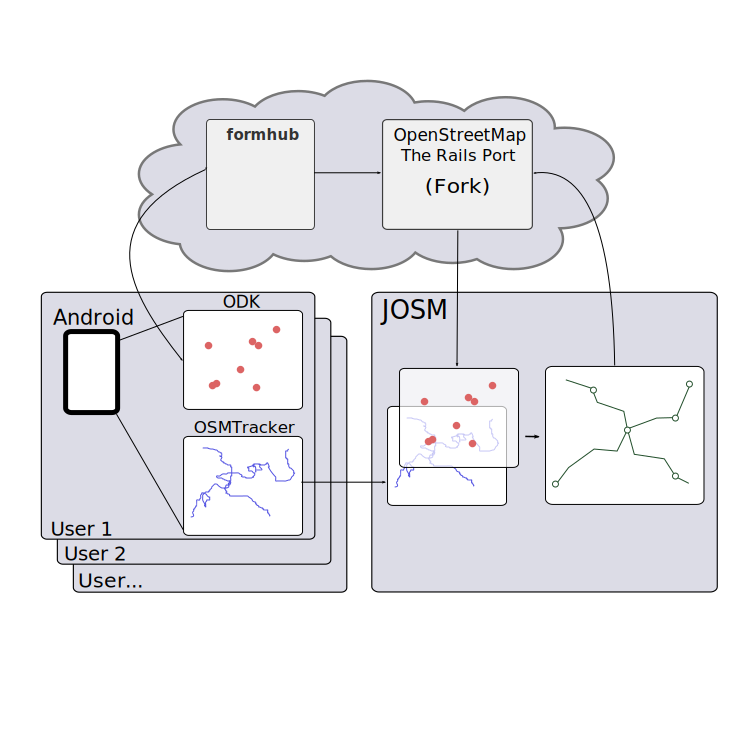
\includegraphics[width=4in,height=3in]{../diagrams/gridmaps-design.png}
\end{frame}

\begin{frame}{OpenStreetMap}
  Virtues:
  \begin{itemize}
  \item[] Topological Model:  Nodes, Ways and Relations
  \item[] Flexibility via Tags
  \item[] Versioned
  \item[] Open
  \item[] Loads of existing data and tools
  \end{itemize}


  \bigskip 

  Issues:
  \begin{itemize}
  \item[] Open license might not fly
  \item[] Technical uncertainty
  \end{itemize}

\end{frame}

\begin{frame}{Approach 1: The Black Hole}
  \begin{center}


  Points via FormHub, Lines via OSMTracker (GPS)
  
  $\Downarrow$ 
  
  Best Practices, Dropbox 
  
  $\Downarrow$ 
  
  Ill-Defined Processing 
  \end{center}

\end{frame}

\begin{frame}{Approach 2: Frankenstein}
  \begin{center}


  Points via FormHub, Lines via OSMTracker (GPS)
  
  $\Downarrow$ 
  
  Synchronization, JOSM 
  
  $\Downarrow$ 
  
  Private Instance of OpenStreetMaps (plngridmaps.modilabs.org)
  \end{center}

\end{frame}

\begin{frame}{Results}


  Numbers (toward our Primary Goal):
  \begin{itemize}
  \item[] 700 km of mv grid digitized
  \item[] Average of about 50 km of mv grid captured per day
  \item[] 2357 km of mv grid managed 
  \end{itemize}
  
  \bigskip 

  The System (toward our Secondary Goal):
  \begin{itemize}
  \item[] Still not pretty, but effective and improvements to come
  \end{itemize}
  
\end{frame}
\end{document}
